\documentclass[conf]{new-aiaa}
\usepackage[utf8]{inputenc}

\usepackage{float}
\usepackage{caption}
\usepackage{multicol}
\usepackage{verbatim}
\usepackage{graphicx}
\usepackage{amsmath}
\usepackage{siunitx}
\usepackage{longtable,tabularx}
\usepackage{fontspec}
\usepackage{minted}

\setmainfont{DejaVu Sans} 
\setmonofont{DejaVu Sans Mono}

\renewcommand\refname{}

\usepackage{hyperref}
\hypersetup{
    colorlinks=false,
    linkcolor=black,
    filecolor=black,      
    urlcolor=cyan,
}

\urlstyle{same}

\graphicspath{{./media/}}

\title{Exploring Invariant Manifolds and Halo Orbits}

\author{Joseph D. Carpinelli
    \footnote{
        Graduate Assistant, 
        Department of Aerospace Engineering, 
        University of Maryland}}
\affil{University of Maryland, College Park, Maryland, 20740}

\begin{document}

\maketitle
\nocite{*}

\begin{abstract}
Low-cost trajectory design has been a subject of research for decades.
Recently, researchers at California Polytechnic State University
studied low-cost trajectory design through the use of invariant
manifolds about Lagrange points in our solar system -- a 
transfer from Earth to Jupiter, with an epoch similar to 
that of Voyager 1, was investigated 
\cite{rund2018interplanetary}. 
This project aims to summarize,
and at times replicate, the core concepts behind this manifold-based 
trajectory design.
A general, analytical 
implementation for a Halo orbit solver is described, and implemented.
A general, numerical implementation for a Halo orbit solver is 
described, and the preliminary code implementation is provided
as a reference. 
This project was completed as part of the University of 
Maryland's ENAE601 (Graduate Astrodynamics) course.
\end{abstract}



\begin{multicols}{2}

\tableofcontents

\section{Motivation}
Halo orbits are stable and periodic
within the Circular Restricted Three Body 
Problem, and can therefore provide satellites the benefit 
of reduced orbit maintenance fuel costs \cite{williams2017targeting}.
For these reasons, Halo orbits have have been
highly researched in recent 
years, and will be utilized in upcoming NASA Artemis missions
\cite{nasa2020artemis}. Separately, low cost trajectories 
are needed to design more efficient space exploration missions.
One such method for low cost trajectory design utilizes 
invariant manifolds about Lagrange points in our solar system --
this method has been shown, in one example, to 
decrease the required transfer $\Delta v$ from
Earth to Jupiter by approximately
$4 \frac{\text{km}}{\text{s}}$ when compared with the $\Delta v$ of a transfer
designed through patched conics \cite{rund2018interplanetary}. 

Halo solutions are not easy to find -- they are often quite
difficult to solve for numerically. 
This topic's complexity, coupled
with it's benefits to future low-cost interplanetary missions,
motivates additional research. 

\section{Introduction}
Periodic, stable orbits are desirable for human spaceflight missions;
eclipse avoidance, positioning for spacecraft communication and space 
science experiments, and data collection can be 
improved through robust orbit stability and periodicity or 
quasi-periodicity \cite{zimovan2020near}. In the Circular Restricted 
Three-body Problem, several families of orbits are known which 
orbit Lagrange points. One such
family of theoretically periodic orbits are 
known as Halo orbits; they are periodic
within the Circular Restricted Three-body Problem, and
quasi-periodic in higher fidelity ephemeris models
\cite{zimovan2020near} \cite{rund2018interplanetary}. This 
periodicity makes Halo orbits attractive candidates for target 
orbits in future space missions. Unfortunately, finding 
Halo orbits is not trivial. An analytical solution, as 
described by Rund, can provide an initial estimate
for a particular Halo orbit \cite{rund2018interplanetary}. However,
numerically propagating this analytical solution will result in 
a non-periodic orbit. A numerical algorithm has been developed to 
iterate from this aperiodic initial orbit to a nearby, periodic orbit 
\cite{rund2018interplanetary} \cite{howell1984three}.

Halo orbits' connection with Lagrange points results in an additional, 
exploitable characteristic: invariant manifolds. Collections of 
trajectories approach, and depart periodic orbits about Lagrange points.
Groups of trajectories which approach the Halo orbit are known 
as stable invariant manifolds, while groups of trajectories which 
depart the Halo orbit are known as unstable invariant manifolds
\cite{rund2018interplanetary}. These trajectories can be utilized by a
spacecraft for low-cost travel along the manifold. 

This project implements the analytical Halo solution in Julia, a scientific
computing language. Several analytical Halo orbits are presented, and 
rough estimates for their numerical solutions are also shown. Note that
neither of these estimates are truly periodic when used as inputs to 
a Circular Restricted Three-body propagator. The summarized numerical
Halo orbit solver must be applied to these initial conditions to find
close-by, truly periodic orbits \cite{rund2018interplanetary} 
\cite{howell1984three}.

\subsection{Outline}
First, the Circular Restricted Three-body Problem (CR3BP) and
Lagrange points will be reviewed, and the added context of 
invariant manifolds will be presented. Next, Halo orbits will be 
introduced, and analytical and numerical methods for solving
Halo orbits will be summarized \cite{rund2018interplanetary}
\cite{howell1984three}. Finally, invariant manifolds about
Halo orbits will be summarized, and low-cost manifold-based 
interplanetary transfer designs will be summarized, as presented
by Rund et al \cite{rund2018interplanetary}.

\section{CR3BP Overview}
The Circular Restricted Three-body Problem is an orbital mechanics 
simplification. Within this domain, a spacecraft of infinitesimal
mass is accelerated by two celestial bodies. 

\subsection{Nondimensionalization}
Initial conditions are
often provided, and propagated, in non-dimensional form. This 
nondimensionalization is completed by dividing all position
units by the distance between the two celestial bodies, and dividing 
all time units by a user-specified duration \cite{vallado2001fundamentals}.
These nondimensionalizations are shown in equations $(1)$ and $(2)$ below,
where subscript $N,s$ denotes the \textit{nondimensional} state of the spacecraft with 
respect to the center of mass of the two celestial bodies (COM), and subscript
$D,s$ denotes the \textit{dimensional} state of the spacecraft with respect to COM. 
The single nondimensional mass parameter is labeled $\mu$, while $\mu_1$ and $\mu_2$ are the
dimensioned mass parameters for the first and second celestial bodies respectively.

\begin{equation}
    \overrightarrow{r}_{N,s} = \overrightarrow{r}_{D,s} \times \frac{1}{DU}
\end{equation}
\begin{equation}
    \overrightarrow{v}_{N,s} = \overrightarrow{v}_{D,s} \times \frac{DT}{DU}
\end{equation}
\begin{equation}
    \mu = \frac{\text{min}(\mu_1, \mu_2)}{\mu_1 + \mu_2}
\end{equation}

\subsection{Equations of Motion}
The nondimensional equations of motion for a spacecraft within the Circular Restricted 
Three-body Problem are shown in equations $(4)$, $(5)$, and $(6)$ below
\cite{vallado2001fundamentals}.

\begin{equation}
\ddot{x} = 2\dot{y} + x - \frac{(1-\mu)(x + \mu)}{r_1^3} - 
    \frac{\mu (x - 1 + \mu)}{r_2^3}
\end{equation}
\begin{equation}
\ddot{y} = -2\dot{x} + y - \frac{(1 - \mu)y}{r_1^3} - \frac{\mu y}{r_2^3}
\end{equation}
\begin{equation}
\ddot{z} = -\frac{(1-\mu)z}{r_1^3} - \frac{\mu z}{r_2^3}
\end{equation}

\begin{equation*}
    r_1 = \sqrt{(x+\mu)^2 + y^2 + z^2}
\end{equation*}
\begin{equation*}
    r_2 = \sqrt{(x+\mu-1)^2 + y^2 + z^2}
\end{equation*}

\section{Lagrange Points}
Lagrange points are equilibrium points within the Circular Restricted Three-body
Problem. There are $5$ equilibrium positions for each CR3BP system
\cite{vallado2001fundamentals}. Their general equations are shown below
\cite{rund2018interplanetary}. All L1, L2, and L3 Lagrange points are of the form 
$\left( x^*, 0, 0 \right)$, and the L4 and L5 Lagrange points are of the form 
$\left( x^*, y^*, 0 \right)$. The Lagrange points for the Earth-Moon CR3BP system
are shown in Figure 1, which replicates Figure 2.2 in Rund et al's \cite{rund2018interplanetary}.

\begin{equation}
    L_1: x - \frac{(1-\mu)}{(x+\mu)^2} + \frac{\mu}{(x + \mu - 1)^2} = 0
\end{equation}
\begin{equation}
    L_2: x - \frac{(1 - \mu)}{(x + \mu)^2} - \frac{\mu}{(x + \mu - 1)^2} = 0
\end{equation}
\begin{equation}
    L_3: x + \frac{(1-\mu)}{(x+\mu)^2} + \frac{\mu}{(x + \mu + 1)^2} = 0
\end{equation}
\begin{equation}
    L_4: x = \frac{1}{2} - \mu,\; y = \frac{\sqrt{3}}{2}
\end{equation}
\begin{equation}
    L_5: x = \frac{1}{2} - \mu,\; y = \frac{-\sqrt{3}}{2}
\end{equation}
    
\begin{figure}[H]
    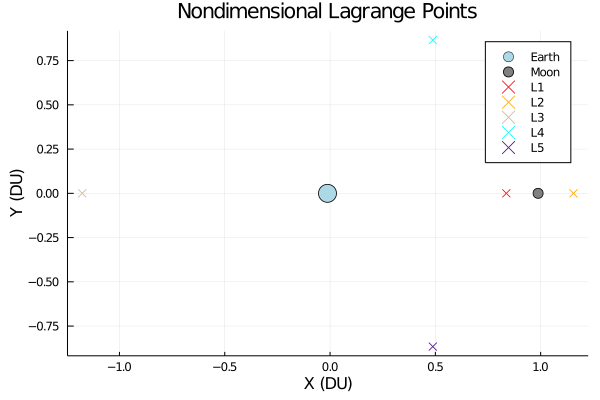
\includegraphics[width=8cm]{fig1}
    \centering
    \captionof{figure}{Earth-Moon Lagrange Points}
\end{figure}

In general, equilibrium positions for nonlinear systems can be stable or unstable. 
Lagrange points are no exception -- perturbing a spacecraft at a stable Lagrange point 
will result in the spacecraft returning to that equilibrium position, while perturbing 
a spacecraft at an unstable Lagrange point will result in the spacecraft continuing to 
diverge from the equilibrium position. Collections of trajectories that 
\textit{diverge from}, or \textit{converge to} Lagrange points are known as 
\textit{manifolds} \cite{rund2018interplanetary}. Figure 2 shows one such example of a 
divergant conditions at an Earth-Moon Lagrange point \cite{rund2018interplanetary}.

\begin{figure}[H]
    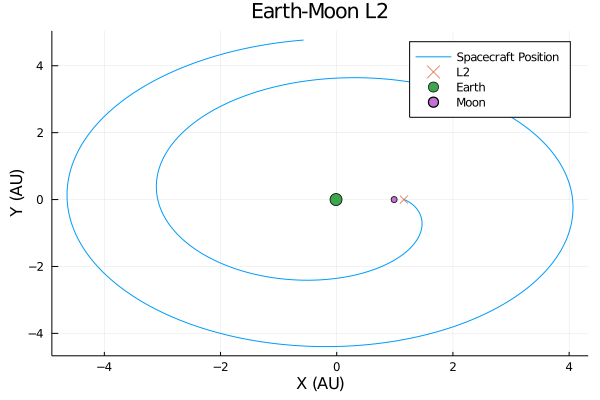
\includegraphics[width=8cm]{fig2}
    \centering
    \captionof{figure}{Divergant Trajectory near Sun-Earth L2}
\end{figure}

\subsection{Manifolds about Lagrange Points}

As previously mentioned, there exist collections of trajectories near Lagrange points 
which approach, and depart each Lagrange point. These collections of trajectories are 
known as manifolds \cite{rund2018interplanetary}. To compute one such trajectory, the 
eigenvectors of the acobian of the state vector at the Lagrange point can be used to 
find perturbations which would place the spacecraft within a manifold 
\cite{rund2018interplanetary}. This use of eigenectors 
is a familiar concept in linear analysis. For a linear system, the eigenvectors
of the zero-input dynamics specify how each state excites each dynamical mode.

The Jacobian of the 
state vector at a Lagrange point will produce two oscillatory pairs of eigenvalues, 
and one pair of real eigenvalues \cite{rund2018interplanetary}. 
The span of the eigenvector corresponding to the 
\textit{larger} real eigenvalue 
represents the perturbations which would move a spacecraft from a Lagrange point to 
an unstable manifold. The span of the eigenvector corresponding to the \textit{smaller} real 
eigenalue represents the perturbations which would move a spacecraft from the Lagrange point
to a stable manifold \cite{rund2018interplanetary}. 
Expressions for the Jacobian of the state vector, and 
perturbing initial conditions for the stable and unstable manifolds near a Lagrange
point are shown below \cite{rund2018interplanetary}.

\begin{equation}
    J = \begin{bmatrix}
        0 & 0 & 0 & 1 & 0 & 0 \\
        0 & 0 & 0 & 0 & 1 & 0 \\
        0 & 0 & 0 & 0 & 0 & 1 \\
        \frac{\partial \ddot{x}}{\partial x} & 
        \frac{\partial \ddot{x}}{\partial y} & 
        \frac{\partial \ddot{x}}{\partial z} & 0 & 2 & 0 \\
        \frac{\partial \ddot{y}}{\partial x} & 
        \frac{\partial \ddot{y}}{\partial y} & 
        \frac{\partial \ddot{y}}{\partial z} & -2 & 0 & 0 \\
        \frac{\partial \ddot{z}}{\partial x} & 
        \frac{\partial \ddot{z}}{\partial y} & 
        \frac{\partial \ddot{z}}{\partial z} & 0 & 0 & 0 \\
    \end{bmatrix}
\end{equation}
\begin{equation}
    X_{\text{STABLE}} = X \pm \epsilon V_{\text{STABLE}}
\end{equation}
\begin{equation}
    X_{\text{UNSTABLE}} = X \pm \epsilon V_{\text{UNSTABLE}}
\end{equation}

\subsection{Orbits about Lagrange Points}
Several families of orbits are known which orbit Lagrange points -- these orbits
are known as Libration orbits \cite{rund2018interplanetary}. Common Libration
orbits include Lyapunov orbits, Halo orbits, and Lissajous orbits; each are briefly 
summarized by Rund, and their descriptions are paraphrased here \cite{rund2018interplanetary}.
Lyapunov orbits are two-dimensional, Halo orbits are periodic and three-dimensional, 
and Lissajous orbits are "quasi-periodic" and three-dimensional 
\cite{rund2018interplanetary}.

\section{Halo Orbit Solutions}
Solving for a Halo orbit is difficult, as the computations are incredibly numerically 
sensitive. An iterative, numerical algorithm has been developed to find a three-dimensional, 
periodic orbit near a provided initial guess \cite{rund2018interplanetary} \cite{howell1984three}.
As Rund shows, an analytical solution can be used as the initial guess \cite{rund2018interplanetary}.

\subsection{Analytical Halo Solution}
Rund outlines an analytical solution for a Halo orbit, given a Z-amplitude and 
non-dimensional mass parameter $\mu$, in great detail in section 3.2 \cite{rund2018interplanetary}.
The algorithm first sets parameter values corresponding to the selected Lagrange point; 
only \textit{L1} and \textit{L2} analytical Halo orbits can be found with this algorithm.
Then, the algorithm plugs these parameters into a general equation of motion. The distance 
from the CR3BP center of mass to the selected Lagrange point must be added to all $x$ values, 
as the algorithm calculates all positions with respect to the selected Lagrange point 
\cite{rund2018interplanetary}.
Rund's explanation is excellant and complete, so it will not be explained in more detail here. 

I implemented this analytical Halo solution with Julia code, as shown in Appendix A.
The analytical solutions can also show the approximate shape of a Halo orbit. The analytical 
algorithm requires an input for Z amplitude of the Halo orbit; 
Rund uses a dimensional Z amplitude as an input, 
and my implementation takes a non-dimensional Z amplitude \cite{rund2018interplanetary}. 
Four examples of analytical solutions for families of Halo orbits are shown in Figure 3, 
Figure 4, Figure 5, and Figure 6. They were computed using my implementation of 
the analytical algorithm \cite{rund2018interplanetary}.

\end{multicols}

\begin{multicols}{2}
\begin{figure}[H]
    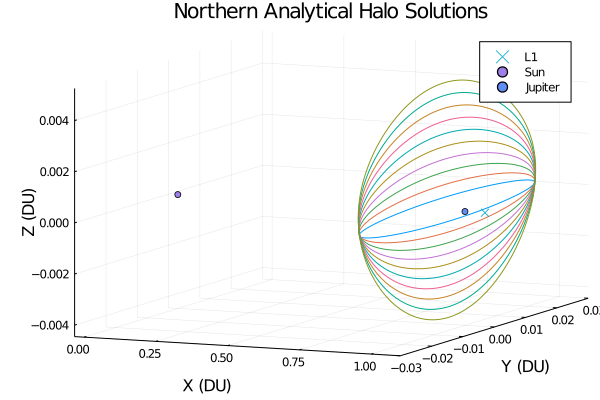
\includegraphics[width=8cm]{fig3}
    \centering
    \captionof{figure}{Northern Halo Orbits about Sun-Jupiter L1}
\end{figure}

\begin{figure}[H]
    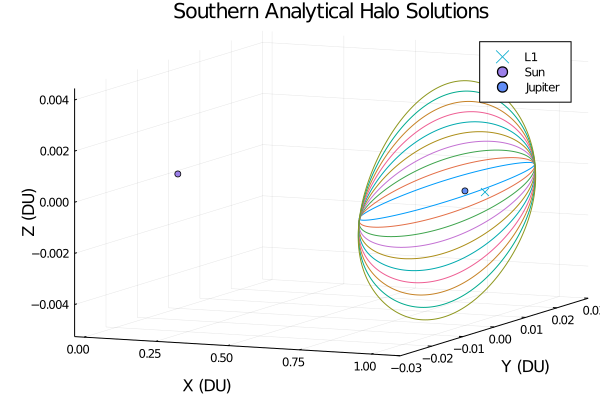
\includegraphics[width=8cm]{fig4}
    \centering
    \captionof{figure}{Southern Halo Orbits about Sun-Jupiter L1}
\end{figure}

\begin{figure}[H]
    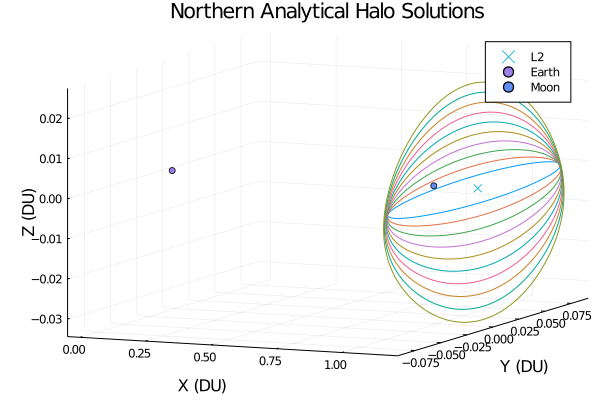
\includegraphics[width=8cm]{fig5}
    \centering
    \captionof{figure}{Northern Halo Orbits about Earth-Moon L2}
\end{figure}

\begin{figure}[H]
    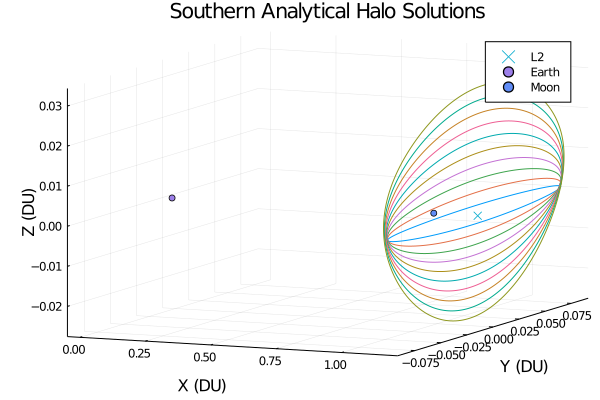
\includegraphics[width=8cm]{fig6}
    \centering
    \captionof{figure}{Southern Halo Orbits about Earth-Moon L2}
\end{figure}

\end{multicols}

\newpage
\begin{multicols}{2}

\subsection{Numerical Halo Solution}

With the $t=0$ step of the analytical Halo solution in-hand, we can use the numerical 
Halo solution to iteratively find a close estimate to a periodic Halo orbit 
\cite{rund2018interplanetary}. This algorithm is presented in literature, 
including by Howell and Rund \cite{howell1984three} \cite{rund2018interplanetary}. 
This algorithm is also presented in Lecture 16 of the University of Maryland's 
Graduate Astrodynamics course, ENAE$601$. For this reason, this section does not 
go into the algorithm in complete detail. Instead, it provides a broad overview.
Rund provides a more complete and detailed explanation \cite{rund2018interplanetary}.

The numerical algorithm involves iterative propagation. Source code in Julia is available
in Appendix B. The analytical algorithm should have produced a state vector of the following form:

\begin{equation*}
\overrightarrow{x} = \begin{bmatrix} x_0^* & 0 & z_0^* & 0 & \dot{y}_0^* & 0 \end{bmatrix}^T
\end{equation*}

We will need to iterate on this initial guess to find a numerically periodic Halo orbit. 
The form of our subsequent guesses will stay the same, but our $x_0$ and $\dot{y}_0$ values 
will change. We could instead choose to change our $z_0$ and $\dot{y}_0$ values, but in 
this description the former option will be used \cite{rund2018interplanetary} 
\cite{howell1984three}. 

To find a new initial state guess, we can use linear analysis techniques to find 
state delta values which will move the solutions in the desired direction. We can 
use the state transition matrix $\Phi$ for this purpose. In the context of the 
Circular Restricted Three-body Problem, the state transition matrix 
$\Phi$ relates the initial state vector to the state vector at each future time $t$ 
\cite{rund2018interplanetary}. The state transition matrix dynamics are described by 
$\dot{\Phi} = F \Phi$, where $F$ is a $6\times 6$ block matrix with zeros at the top left,
the identity matrix at the top right, the Hessian (matrix of second partial derivatives)
of the potential energy of the spacecraft at the bottom left, and a constant matrix at 
the bottom right \cite{rund2018interplanetary}.

\begin{equation}
    F = \begin{bmatrix} 0 & I_3 \\ U_{XX} & 2\Omega \end{bmatrix}
\end{equation}
\begin{equation}
    \Omega = \begin{bmatrix} 0 & 1 & 0 \\ -1 & 0 & 0 \\ 0 & 0 & 0  \end{bmatrix}
\end{equation}
\begin{equation}
    U_{XX} = \begin{bmatrix} 
        \frac{\partial^2 U}{\partial x \partial x} & 
        \frac{\partial^2 U}{\partial x \partial y} & 
        \frac{\partial^2 U}{\partial x \partial z} & \\
        \frac{\partial^2 U}{\partial y \partial x} & 
        \frac{\partial^2 U}{\partial y \partial y} & 
        \frac{\partial^2 U}{\partial y \partial z} & \\
        \frac{\partial^2 U}{\partial z \partial x} & 
        \frac{\partial^2 U}{\partial z \partial y} & 
        \frac{\partial^2 U}{\partial z \partial z} & \\
    \end{bmatrix}
\end{equation}

With the equations above defined, we have all we need to complete the numerical algorithm.
The initial state transition matrix is set to the identity matrix, and each row is appended 
to the state vector. As a result, the total state vector for this numerical integration 
contains $42$ variables. We numerically integrate the initial state vector until 
the solution crosses the $x-z$ axis (that is, when $y = 0$). We then add the following 
state deltas to our initial condition, and repeat the procedure until the values $\dot{x}$ and 
$\dot{z}$ are within some tolerance near zero \cite{rund2018interplanetary}. After this 
procedure finishes, we should be left with an initial condition vector for a periodic Halo orbit.
This orbit may still diverge after several periods of numerical integration, depending on 
how small our numerical tolerance was set \cite{rund2018interplanetary}.

\begin{equation}
    \delta \dot{x} = -\dot{x},\; \delta \dot{z} = -\dot{z}
\end{equation}
\begin{equation}
    \begin{bmatrix} \delta x_0 \\ \delta \dot{y}_0 \end{bmatrix} = 
    \left( \begin{bmatrix} \Phi_{4 1} & \Phi_{4 5} \\ \Phi_{6 1} & \Phi_{6 5} \end{bmatrix} - 
    \frac{1}{\dot{y}} \begin{bmatrix} \ddot{x} \\ \ddot{z} \end{bmatrix} \right)^{-1} 
    \begin{bmatrix} \delta \dot{x} \\ \delta \dot{z} \end{bmatrix}
\end{equation}

\section{Invariant Manifolds}

\subsection{Overview}

Each point along the periodic Halo orbit is connected with an unstable and stable 
invariant manifold -- this manifold is a collection of spacecraft trajectories 
which converge to the point on the Halo orbit (stable manifold), or diverge from 
the point on the Halo orbit (unstable manifold) \cite{rund2018interplanetary}.
We could calculate the eigenvectors of the Jacobian at each time step to give us the 
range of perturbations which would shift the spacecraft onto the manifold, as previously 
discussed. As Rund points out, this is very computationally expensive. Instead, we can 
use the monodromy matrix -- the state transition matrix after one period $T$ 
\cite{rund2018interplanetary}.

\subsection{Algorithm}

To find the range of perturbations (in state space) which will shift the spacecraft 
onto the unstable or stable manifolds at each time step along the Halo orbit, 
we simply need to numerically integrate the full $42$ element state vector (with $\Phi$ set
to the identity matrix as an initial value) for one full period. We then note the 
monodromy matrix is equivalent to the final state transition matrix. The eigenvector 
associated with the maximum eigenvalue of the monodromy matrix, $V^U$, is used to find perturbations 
to reach the unstable manifold, and the eigenvector associated with the minimum eigenvalue, $V^S$,
is used to find perturbations to reach the stable manifold 
at each time step $i$, and some small scalar perturbation magnitude 
$\epsilon$ \cite{rund2018interplanetary}. This is shown in equations $(20)$ through $(24)$.

\subsection{Usage}

Once the perturbing state delta has been found for each time step, and for both the 
unstable and stable invariant manifolds, we can numerically integrate many trajectories 
along each point in the Halo orbit to visualize the stable and unstable invariant manifolds. 
This can be seen in Rund's Figure 3.6 \cite{rund2018interplanetary}. Trajectories within
unstable manifolds are propagated forward in time, and trajectories within stable manifolds are 
propagated backwards in time. As Rund shows, these invariant manifolds about Halo 
orbits can be utilized to form low-cost transfers from one Halo orbit to another 
\cite{rund2018interplanetary}. Substantial $\Delta v$ savings are reported when 
compared with traditional trajectory design methods; Rund's Masters Thesis provides 
more detail \cite{rund2018interplanetary}.

\begin{equation}
    V_i^{S} = \Phi(t_0 + t_i, t_0) V^S
\end{equation}
\begin{equation}
    V_i^{U} = \Phi(t_0 + t_i, t_0) V^U
\end{equation}
\begin{equation}
    X_i^{S} = X_i \pm \epsilon \frac{V_i^S}{|V_i^S|}
\end{equation}
\begin{equation}
    X_i^{U} = X_i \pm \epsilon \frac{V_i^U}{|V_i^U|}
\end{equation}

\begin{equation}
M = \Phi(t_0 + T, t_0)
\end{equation}

\section{Conclusion}
Halo orbits have many desirable properties \cite{zimovan2020near} \cite{rund2018interplanetary}.
They are also incredibly difficult to find numerically with high precision. A method for 
finding analytical solutions for Halo orbits was summarized and implemented 
\cite{rund2018interplanetary}. A method for iterating on this analytical initial guess 
to find a numerically periodic Halo orbit was summarized and implemented, though 
the implemented code is not fully functional \cite{rund2018interplanetary} \cite{howell1984three}.

Common linear analysis techniques can be used to find manifolds about Halo orbits
\cite{rund2018interplanetary} \cite{howell1984three}. These 
manifolds can then be utilized to form low-cost transfers between Halo orbits 
\cite{rund2018interplanetary}. Future work includes fixing the numerical Halo solver code,
and exploring potential cost benefits for different interplanetary transfers.

\end{multicols}

\section{References}
\bibliography{sources}

\newpage
\section{Appendix}

Code to evaluate analytical and numerical Halo solutions are shown below. Only the 
analytical function is working at the time of writing. If the unicode characters in 
variables names are cutoff in your PDF version of this document, you can find 
the same code on GitHub at \href{https://github.com/cadojo/UnitfulAstrodynamics.jl/blob/dev/src/ThreeBody/ThreeBodyCalculations.jl}{cadojo/UnitfulAstrodynamics.jl}. 
The numerical function, "halo", currently has bugs that have not yet been resolved.
All orbits produced by this function seem to be shifted such that they are 
no longer encircling the Lagrange point.  

\inputminted[breaklines=true]{julia}{../../../../../../FOSS/UnitfulAstrodynamics/src/ThreeBody/Halo.jl}


\end{document}